% Include at a fixed width: scaling DOWN would push the
% in-figure type below the 9pt floor the artwork guide sets.
\begin{figure}[t]
  \centering
  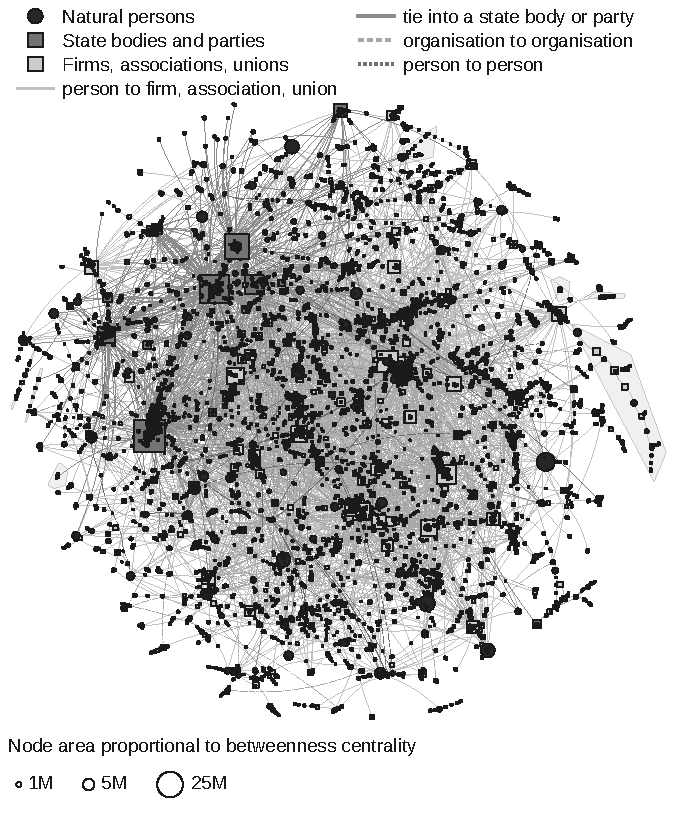
\includegraphics[width=4.5in]{fig15_brokerage_network_all.pdf}
  \caption{\textbf{The Tunisian elite network.}
  Node area is proportional to betweenness centrality. Every entity and every tie is drawn
  and none is named: 23,274 entities joined by
  31,457 ties. The graph falls into 1 components,
  so the largest is laid out by force and the remaining 0
  fragments are packed into rings around it -- the positions of
  disconnected nodes are arbitrary, and a force layout spread these
  fragments over three quarters of the canvas, giving arbitrary structure
  the visual weight. Betweenness is exactly zero for 20,381 of them
  (88\%), which a strictly proportional area
  would render invisible, so area is proportional above a floor of
  0.9pt. Selection is therefore on
  the quantity the node areas encode. Ties are
  undirected and undated, pooling shareholding, board and governing-body
  membership, kinship, party and parliamentary structures, and the seed
  roster, over 1957--2026.
  The composition is 8,009 natural persons, 217 state bodies
  and parties, and 15,048 firms, associations and unions.}
  \label{fig:fig15_brokerage_network_all}
\end{figure}

% ---------------------------------------------------------------------
% Accessibility description (APSR requires one; WCAG 2.1 AA)
% ---------------------------------------------------------------------
% A node-link diagram of 23274 entities connected by
% 31457 lines, drawn in greyscale. Circles are natural
% persons, squares are organisations; darker fills are state bodies and
% parties, lighter fills are firms, associations and unions. The area of
% each shape is proportional to its betweenness centrality, so the
% entities that lie on the most shortest paths appear largest. A small
% number of very large nodes sit at the centre of the diagram and connect
% several otherwise separate dense clusters of smaller nodes. No entity is
% named on the figure. A size key at the lower left gives
% reference areas in millions.
